\documentclass[conference]{IEEEtran}
\usepackage{cite}
\usepackage{amsmath,amssymb,amsfonts}
\usepackage{algorithmic}
\usepackage{graphicx}
\usepackage{siunitx}
\usepackage{textcomp}
\usepackage{xcolor}
\usepackage{multirow}
\usepackage{url}
\usepackage{listings}
\usepackage{epstopdf}
\usepackage{subcaption}
\usepackage[inkscapeformat=png]{svg}
\usepackage[font=small,labelfont=bf]{caption}

\epstopdfDeclareGraphicsRule{.gif}{png}{.png}{convert gif:#1 png:\OutputFile}
\AppendGraphicsExtensions{.gif}

\begin{document}

\title{Single-Depot Multiple Travelling Salesman Problem optimisation using a Genetic algorithm and a Particle Swarm Optimisation algorithm}

\author{\IEEEauthorblockN{Mihai Bojescu}
\IEEEauthorblockA{\textit{Master in Artificial Intelligence and optimisation} \\
\textit{Faculty of Computer Science of University ``Alexandru Ioan Cuza'' of Iași}\\
Iași, Romania \\
bojescu.mihai@gmail.com}
}
\maketitle

\begin{abstract}
    This document contains a study on optimising the Single-Depot, Multiple Travelling Salesman Problem using a combinatorial
    Genetic algorithm and a combinatorial Partile Swarm Optimisation algorithm. The studied problem is presented in detail, along
    with the algorithms, their inner workings, diagrams, hyperparameters, timings and results. The study was conducted on the eil51,
    berlin52, eil76, rat99 datasets with 2, 3 and 5 salesmen.
\end{abstract}

\begin{IEEEkeywords}
Single-Depot Multiple Travelling Salesman Problem, Genetic algorithm, Particle Swarm Optimisation algorithm, SD-MTSP,
GA, PSO, TSPLIB, optimisation, combinatorial function optimisation.
\end{IEEEkeywords}

\section{Introduction}
The Multiple Traveling Salesman Problem (MTSP) is a generalization of the well-known Traveling Salesman Problem (TSP),
where multiple salesmen are involved to visit a given number of cities exactly once and return to the initial position
with the minimum traveling cost. MTSP is highly related to other optimisation problems such as Vehicle Routing Problem (VRP)
and Task Assignment problem \cite{b1}. In this study, we will optimise the Single-Depot, Multiple Travelling Salesman Problem,
which is a variation of MTSP.

Genetic algorithms were proposed by John Holland in 1973 after many years of studying the idea of simulating evolution.
These algorithms model genetic inheritance and the Darwinian struggle for survival. Together with two other directions: evolutionary
strategies and evolutionary programming, they form the class of evolutionary algorithms \cite{b2}. In this study, we will
be using a combinatorial GA.

Particle Swarm Optimisation (PSO) algorithm is one of the most well-regarded algorithm in the literature of stochastic optimisation
approaches. It belongs to the family of swarm-based techniques and is a population-based algorithm. As GA and ACO, it is
of the most well-regarded algorithm in the literature. There are different versions of this algorithm in the literature
to solve constrained, dynamic, discrete, multi-objective, multi-modal, and many-objective problems \cite{b3}. In this study,
we will be using a modified PSO which can work with combinatorial problems.

This paper will apply the algorithms stated above in order to optimise the problem stated above.

\section{Single-Depot, Multiple Travelling Salesman Problem}
MTSP is one of the most important optimisation problems, and it has been applied in several real-life scenarios. Depending
on the application requirements, the salesmen in MTSP can be represented by ground vehicles such as robots or trucks, or by
flying vehicles such as Unmanned Aerial Vehicles (UAVs) known also as drones. Whereas the cities to be visited by the salesmen
can have different representations, such as customers in transportation and delivery services, sensor nodes for Wireless Sensor
Networks data collection, targets in military applications, victims in emergency missions and critical sites in disaster management
applications \cite{b1}.

MTSP is a multi-goal problem. Given $n$ salesmen and $m$ cities, the problem seeks to optimise the following two goals:
\begin{enumerate}
    \item To minimise the total tour cost of $n$ salesman that have to visit $m$ cities, at the end returning to the ``home'' city
    \item To minimise the tour cost of $n$ salesmen that have to visit $m$ cities, at the end returning to the ``home'' city
\end{enumerate}

Mathematically, MTSP can be expressed in the following way: Given $n \in \mathbb{N}$ salesmen and $m \in \mathbb{N}$ cities,
the tour definition

\begin{equation}
    tour_i = \{city | city \in \{1, ..., m\}\}, i \in \{1, ..., n\}
\end{equation}

\begin{equation}
    tour_i \cap tour_j = \emptyset, i \ne j, i \in \{1, ..., n\}, j \in \{1, ..., n\}
\end{equation}

\begin{equation}
    \bigcup_{i = 1}^{n} tour_i = \{1, ..., m\}
\end{equation}

\begin{equation} \label{tour maximum length}
    |tour| \leq \lfloor \frac{m - 1 + n}{n} + 1 \rfloor
\end{equation}

and the cost function

\begin{multline} \label{cost function}
    cost(tour) = (\sum_{i = 1}^{k - 1} distance^2(city_{i}, city_{i+1})) + \\
    distance^2(city_k, city_1), k = |tour|
\end{multline}


find a combination of tours such that

\begin{equation}
    minimise(\sum_{i = 1}^{n} cost(tour_i))
\end{equation}

and

\begin{equation}
    minimise(cost(tour_i)), \forall i \in \{1, ..., n\}
\end{equation}

are satisfied.

The MTSP problem can be optimised using multiple heuristic algorithms: Artificial Neural Networks (ANNs), Simulated
Annealing algorithms (SAs), Particle Swarm Optimisation algorithms (PSOs), Genetic algorithms (GAs), Ant Colony Optimisation
algorithms (ACOs) etc. \cite{b4}.


\section{Genetic Algorithm}

\subsection{Introduction}
In literature, Genetic Algorithms are regarded as highly effective for optimising the MTSP, thus they are extensively used (Xu
et al. 2018) due to their convergence speed, their main drawback being their high dependence on a well-generated, diverse initial
population.

Multiple Genetic Algorithms were proposed, ranging from their chromosome representation and used genetic operators.

For chromosome representations, Tang et al. (2000) suggested a one-chromosome representation for optimising MTSP and was
used for tackling the hot rolling production scheduling problem. Carter and Ragsdale (2006) proposed a two-part chromosome
representation and relevant operators. Brown et al. (2007) proposed a one-chromosome and two-chromosome representation, while
Yuan et al. (2013) proposed another two-part chromosome representation algorithm.

As for genetic operators, many used simple swap, slide and reverse-swap operators for the mutation operator. For the crossover
operator, Király and Abonyi (2011) proposed a two-point crossover operator, Lo et al (2018) proposed a edge-recombination crossover
operator, Sedighpour et al. (2012) proposed an order crossover operator, and Singh et al. (2018) proposed a distance-preserving
crossover operator for solving the MTSP.

\subsection{Hyperparameters}
In this paper, the following hyperparameters were chosen for the genetic algorithm:
\begin{enumerate}
    \item population size = 100
    \item generations = 2000
    \item mutation probability = 0.1
\end{enumerate}

\subsection{Population generation} \label{Genetic algorithm population generation}
In this paper, a population of 100 individuals was generated randomly and was segmented in multiple tours with their maximum
length according to formula \ref{tour maximum length}, in order to match the tour sizes in the provided datasets \cite{b5}.

\subsection{Chromosome representation}
In this paper, a one-chromosome representation was used, where each chromosome was wrapped in an class named ``Individual''
that handled its own fitness calculations using formula \ref{cost function}. Each ``Individual'' represents a full solution
for the MTSP. The tours in the ``Individual'' are entities of type \texttt{t.List[t.List[int]]} with their home depot omitted,
and the fitness value of the solution is represented as a \texttt{float} variable. An example of an individual can be found
in the code listing below.

\begin{lstlisting}[caption=Example of individual,captionpos=b]
Individual(
    genes=[
        [39, 47,  4, 24, 25, 26, 27, 11,
         50, 32, 42,  9,  8,  2, 48, 34,
         43, 15, 28, 49, 19, 22, 30, 20],
        [46, 12, 13, 51, 10,  3,  5, 14,
         37, 23, 45, 36, 38, 35, 33, 21,
         31, 44,  7, 40, 18, 17, 16,  6,
          1, 41, 29]
    ],
    fitness=10361.20300592295
)
\end{lstlisting}

\subsection{Algorithm}
The base algorithm was not modified, as it did not need any modifications performed. Mainly, the only change needed was to
perform dependency injection on the operators, in order to ensure that the algorithm respects the Open-Closed principle.

\subsection{Selection operator}
In this paper, a tournament selection operator was used, where $size(tournament) = 10$, thus from a random selection of 10
individuals, only the best one is picked. There were attempts to use the roulette wheel selection, but the results of using
the tournament selection operator were better.

\subsection{Crossover operator}
For the crossover operator, the distance-preserving crossover operator was used as described by Singh et al. (2018) \cite{b7}. The operator,
originally used on chromosomes with two-part representation, was \textit{trivially} adapted to work using one-chromosome
representations. In order for the operator to be used, an encoder was created that, given a segmentation, can encode the
tours from a \texttt{t.List[t.List[int]]} to a \texttt{t.List[int]} and decode them back.

The operator, given parents $parent_{1}$ and $parent_{2}$ produces children $child_{1}$ and $child_{2}$ in the following manner:
\begin{enumerate}
    \item Encode the tours of $parent_{1}$ into a list of ints, $parent_{1}^{e}$
    \item Encode the tours of $parent_{2}$ into a list of ints, $parent_{2}^{e}$
    \item Create child $child_{1}^{e}$ of length $|parent_{1}^{e}|$
    \item Create child $child_{2}^{e}$ of length $|parent_{2}^{e}|$
    \item Copy last gene of $parent_{2}^{e}$ into first gene of $child_{1}^{e}$
    \item Copy last gene of $parent_{1}^{e}$ into first gene of $child_{2}^{e}$
    \item Copy first gene of $parent_{2}^{e}$ into last gene of $child_{1}^{e}$
    \item Copy first gene of $parent_{1}^{e}$ into last gene of $child_{2}^{e}$
    \item For $i = \{1, ..., |parent_{1}^{e}|\}, j = \{2, ..., |parent_{1}^{e}| - 1\}$:
    \begin{enumerate}
        \item If $i^{th}$ gene of $parent_{2}^{e}$ is equal to $j^{th}$ gene of $parent_{1}^{e}$, then copy $j^{th}$ gene of
        $parent_{2}^{e}$ into $j^{th}$ gene of $child_{1}^{e}$
        \item If $i^{th}$ gene of $parent_{1}^{e}$ is equal to $j^{th}$ gene of $parent_{2}^{e}$, then copy $j^{th}$ gene of
        $parent_{1}^{e}$ into $j^{th}$ gene of $child_{2}^{e}$
    \end{enumerate}
    \item Decode $child_{1}^{e}$ into the tours for $child_{1}$
    \item Decode $child_{2}^{e}$ into the tours for $child_{2}$
\end{enumerate}

An example can be found in the figure below:

\begin{figure}[h]
    \centering
    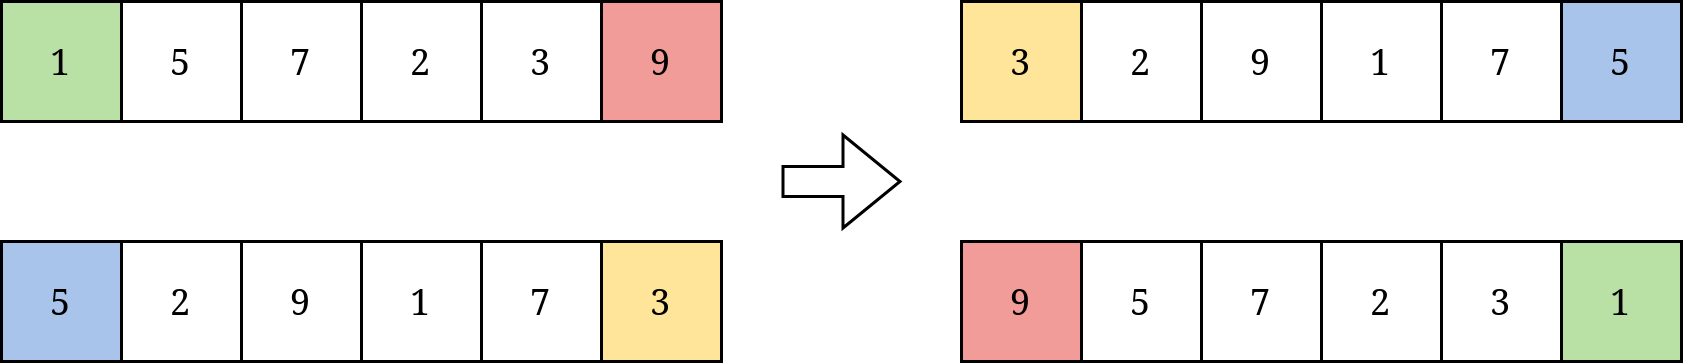
\includegraphics[width=0.45\textwidth]{images/crossover.png}
    \caption{Crossover operator}
\end{figure}


The justification behind this crossover strategy depends on the idea that the city in optimal/suboptimal tour takes place
in the same location \cite{b6}.

\subsection{Mutation operator} \label{Genetic algorithm mutation operator}
The mutation operator in this paper is comprised of 3 operations, each executed according to the mutation probability hyperparameter:

\begin{enumerate}
    \item Swap operation
    \item Slide operation
    \item Reverse-swap operation
\end{enumerate}

The swap operation, randomly picking two position $a$ and $b$ with $a, b \leq |genes_{child}|$, performs a simple swap between
gene $a$ and gene $b$ of the child. A sample can be found in figure \ref{Swap operation}
below.

\begin{figure}[h]
    \centering
    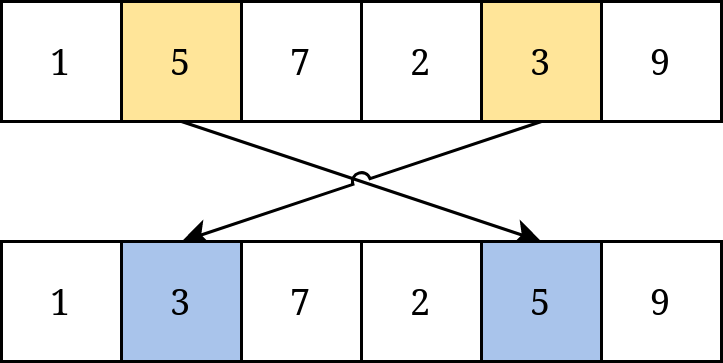
\includegraphics[width=0.20\textwidth]{images/mutation 1.png}
    \caption{Swap operation} \label{Swap operation}
\end{figure}

The slide operation, randomly picking two position $a$ and $b$ with $a, b \leq |genes_{child}|$, moves gene $a$ to gene
$b$ and slides each gene before gene $b$ one step before. A sample can be found in figure \ref{Slide operation}
below.

\begin{figure}[h]
    \centering
    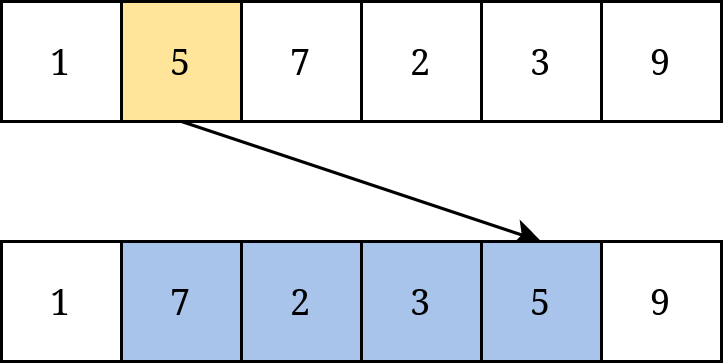
\includegraphics[width=0.20\textwidth]{images/mutation 2.png}
    \caption{Slide operation} \label{Slide operation}
\end{figure}

The reverse-swap operation, randomly picking two position $a$ and $b$ with $a, b \leq |genes_{child}|$, reverses the genes
array between gene $a$ and gene $b$, including gene $a$ and gene $b$. A sample can be found in figure \ref{Reverse-swap operation}
below.

\begin{figure}[h]
    \centering
    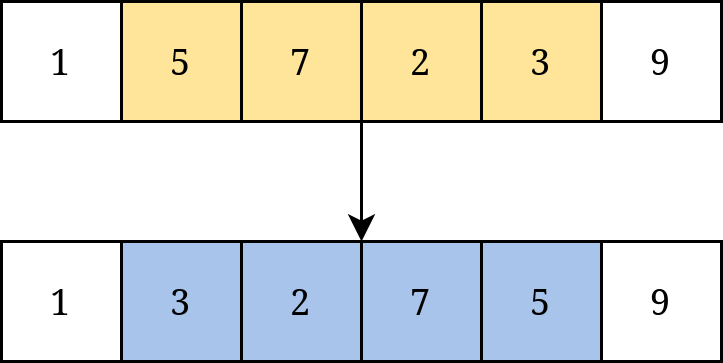
\includegraphics[width=0.20\textwidth]{images/mutation 3.png}
    \caption{Reverse-swap operation} \label{Reverse-swap operation}
\end{figure}

\section{Particle Swarm Optimisation}

\subsection{Introduction}
PSO is a wonderful optimisation technique, inspired from the flocking behaviour of birds. It was successfully applied in
many fields that implied numerical function optimisations, fields such as industry engineering, civil engineering, energy
systems engineering, electrical engineering and geology engineering \cite{b8}.

In order to be able to apply PSO to MTSP, several changes needed to be performed. The motion aspect was transformed in order
to be applied for combinatorial functions. This will be detailed in the following section, \ref{PSO motion subsection}.

\subsection{From motion to operators} \label{PSO motion subsection}
PSO is well known for being an algorithm which incorporates motion. The particles ``move'' through the problem space, exploring
it according to their hyperparameters:

\begin{enumerate}
    \item inertia
    \item their tendency towards their personal best
    \item their tendency towards their global best
\end{enumerate}

Along their some randomly parameters chosen at each step, in order to explore the space better.

The above statement works perfectly for numerical functions, but is troublesome for combinatorial functions. The values needing
to be discrete, can cause a lot of aproximation errors, thus, in this paper, the concepts were replaced:

\begin{enumerate}
    \item For velocity and inertia, a 2-opt algorithm was used instead
    \item For tendency towards a particle's personal best, the path-relinker from the GRASP algorithm was used
    \item For tendency towards a particle's global best, the path-relinker from the GRASP algorithm was used
    \item For randomness, the same swap, slide and reverse-swap operator from the Genetic Algorithm (section \ref{Genetic algorithm mutation operator})
    was used
\end{enumerate}

\subsection{Hyperparameters}
In this paper, the following hyperparameters were chosen for the Particle Swarm Optimisation algorithm:
\begin{enumerate}
    \item population size = 100
    \item iterations = 100
    \item 2-opt probability = 0.2
    \item path-relinker towards personal best probability = 0.4
    \item path-relinker towards global best probability = 0.3
    \item swap probability = 0.1
\end{enumerate}

\subsection{Population generation}
Same as the Genetic algorithm in section \ref{Genetic algorithm population generation}, the population was generated randomly,
without any changes.

\subsection{Algorithm}
The algorithm performs the following steps, as described in the bibliography \cite{b8}:
\begin{enumerate}
    \item $\forall individual \in population$:
    \begin{enumerate}
        \item Select a random number $k, k \in \{1, 2, 3, 4\}$ respecting the input hyperparameters
        \item If $k = 1$, run the 2-opt algorithm operator on the $individual$
        \item If $k = 2$, run the path-relinker algorithm operator on the $individual$, with their $individual$'s personal best as the guiding solution
        \item If $k = 3$, run the path-relinker algorithm operator on the $individual$, with the global best as the guiding solution
        \item If $k = 4$, run the swap operator on $individual$
    \end{enumerate}
    \item Update the individual best of each individual
    \item Update the global best
\end{enumerate}

A flow diagram of the algorithm can be found in figure \ref{Combinatorial PSO algorithm} below:

\begin{figure}[h]
    \centering
    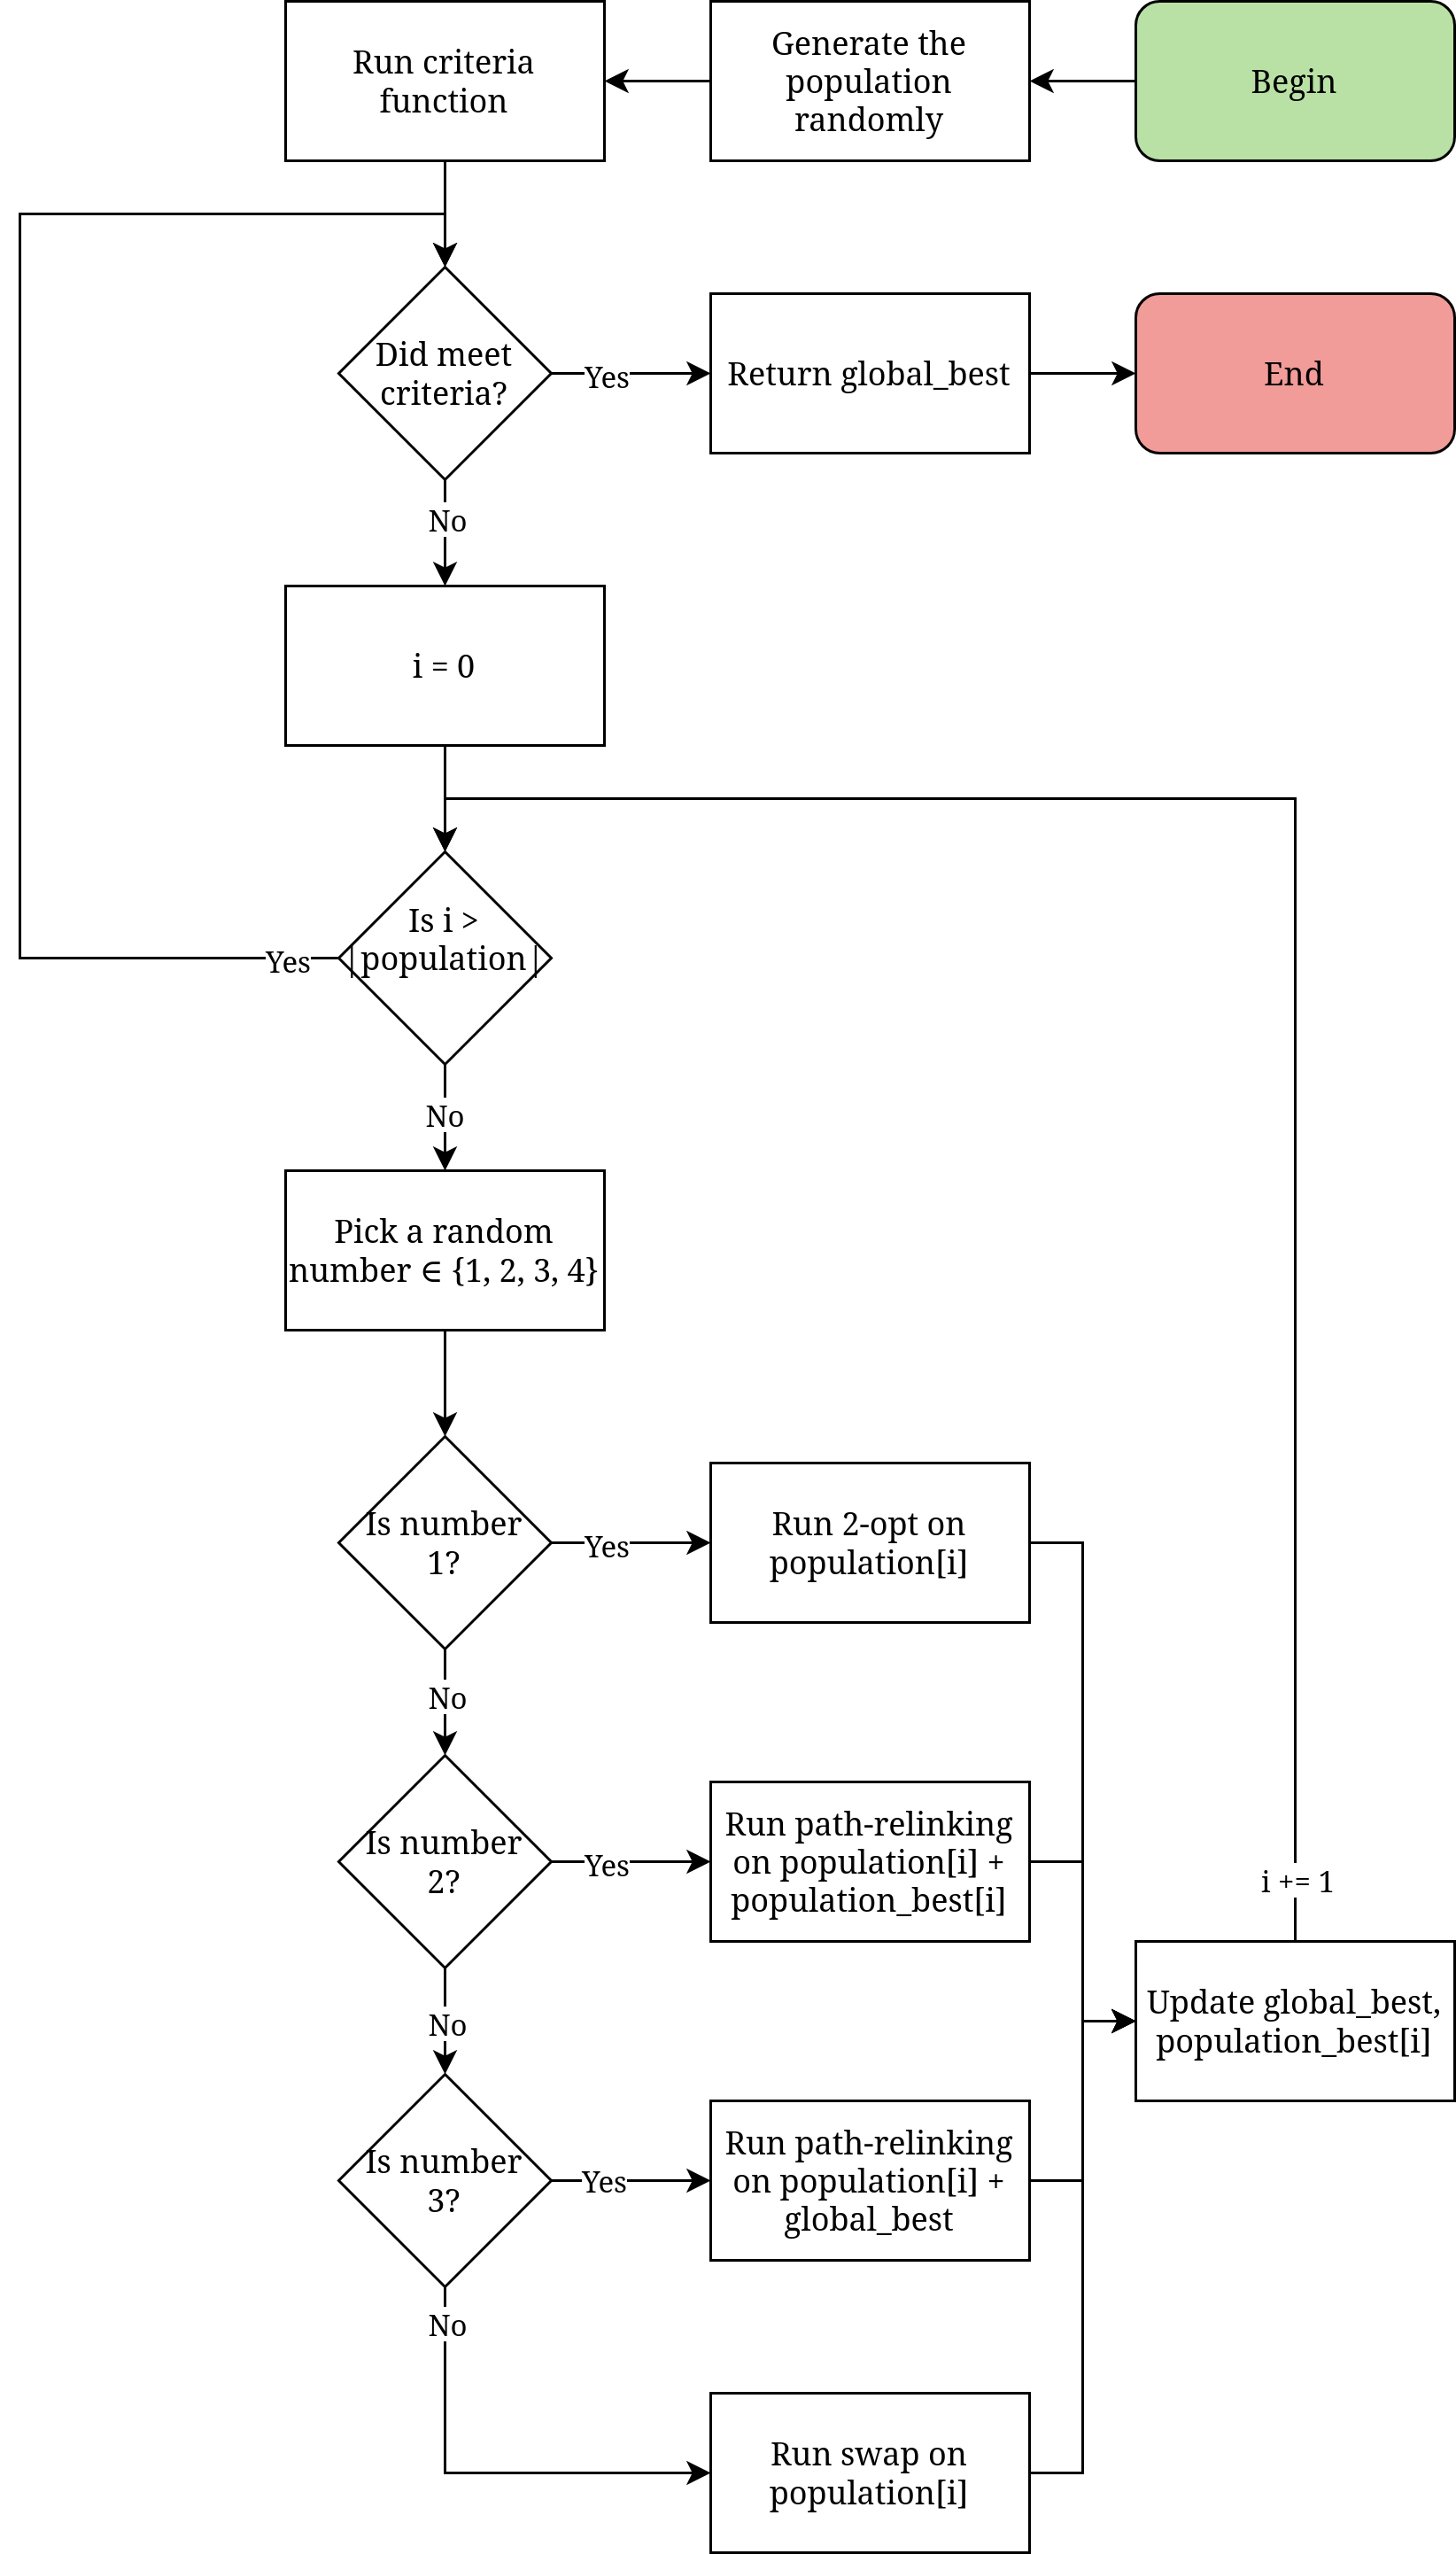
\includegraphics[width=0.39\textwidth]{images/pso.png}
    \caption{Combinatorial PSO algorithm} \label{Combinatorial PSO algorithm}
\end{figure}

\subsection{2-opt algorithm operator}
The 2-opt algorithm is a local search algorithm first proposed by Croes in 1958, with the bassic moves suggested by Flood.
It aims to recombine edges in the MTSP tour such that better alternatives are found, until no more updates can be performed.
At each, the algorithm checks wether the objective function returned better result than the currently known one \cite{b8}.
The main idea of the algorithm is to ensure that there are no edges in a route that cross over themselves \cite{b9}.

A diagram showing how the algorithm works is provided in figure \ref{2-opt algorithm sample} below.

\begin{figure}[h]
    \centering
    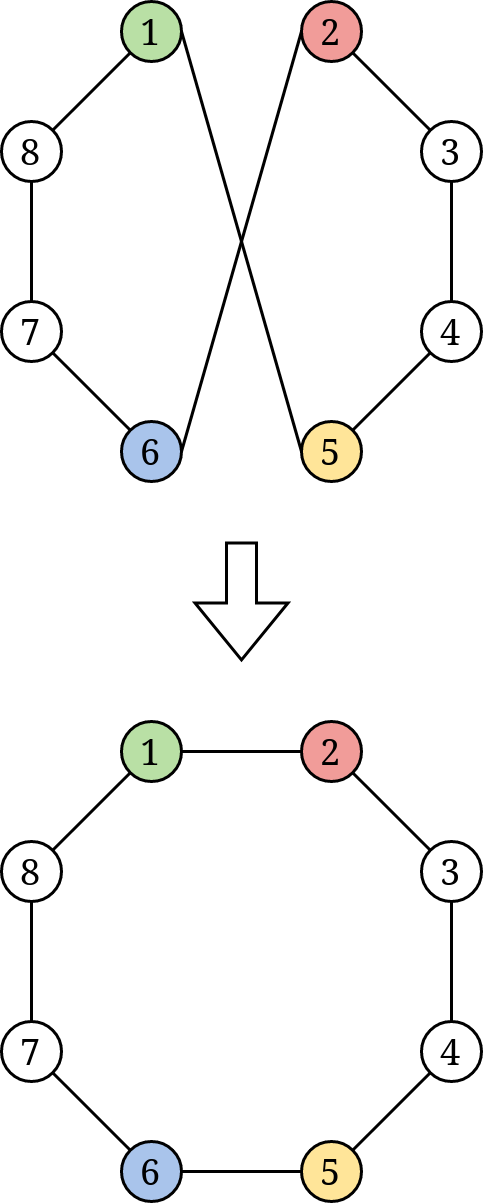
\includegraphics[width=0.175\textwidth]{images/2-opt.png}
    \caption{2-opt algorithm sample} \label{2-opt algorithm sample}
\end{figure}

This operator aims to replace a PSO's particle's velocity and independent movement.

\subsection{Path-relinker algorithm operator}
The relinking procedure (Glover et al. 2004) is used to generate new solutions by exploring trajectories confined in the neighbourhood space
that connect high-quality solutions. The solution that begins the path is named the initiating solution, while the solution
ending the path is named the guiding solution \cite{b10}.

In literature, multiple variants can be found for this procedure, categorised by how the path is built between the initiating
solution and the guiding solution: forward relinking, backward relinking, backward-and-forward relinking, relinking (Glover
et al. 1996, implemented by Resende and Ribeiro 2010a), greedy randomised adaptive path relinking and evolutionary path-relinking \cite{b11}.
Each variant has its own set of advantages and disadvantages. In the computational experiments performed by Aiex et al. (2005),
backward relinking stood out as better performing than forward relinking, and had equivalent performance as backward-and-forward relinking,
but with lower computational costs \cite{b11}.

In this paper, the backward path relinking was used. Thus, the initial solution was the current individual's position and the
guiding solution was - depending on the function call - the individual's best position or the global best position.

A sample can be found in figure \ref{Path-relinker algorithm sample} below. When step 4 is reached, no other better paths moving
towards the given guiding solution could be found, thus the algorithm returns the solution built at step 4.

\begin{figure}[h]
    \centering
    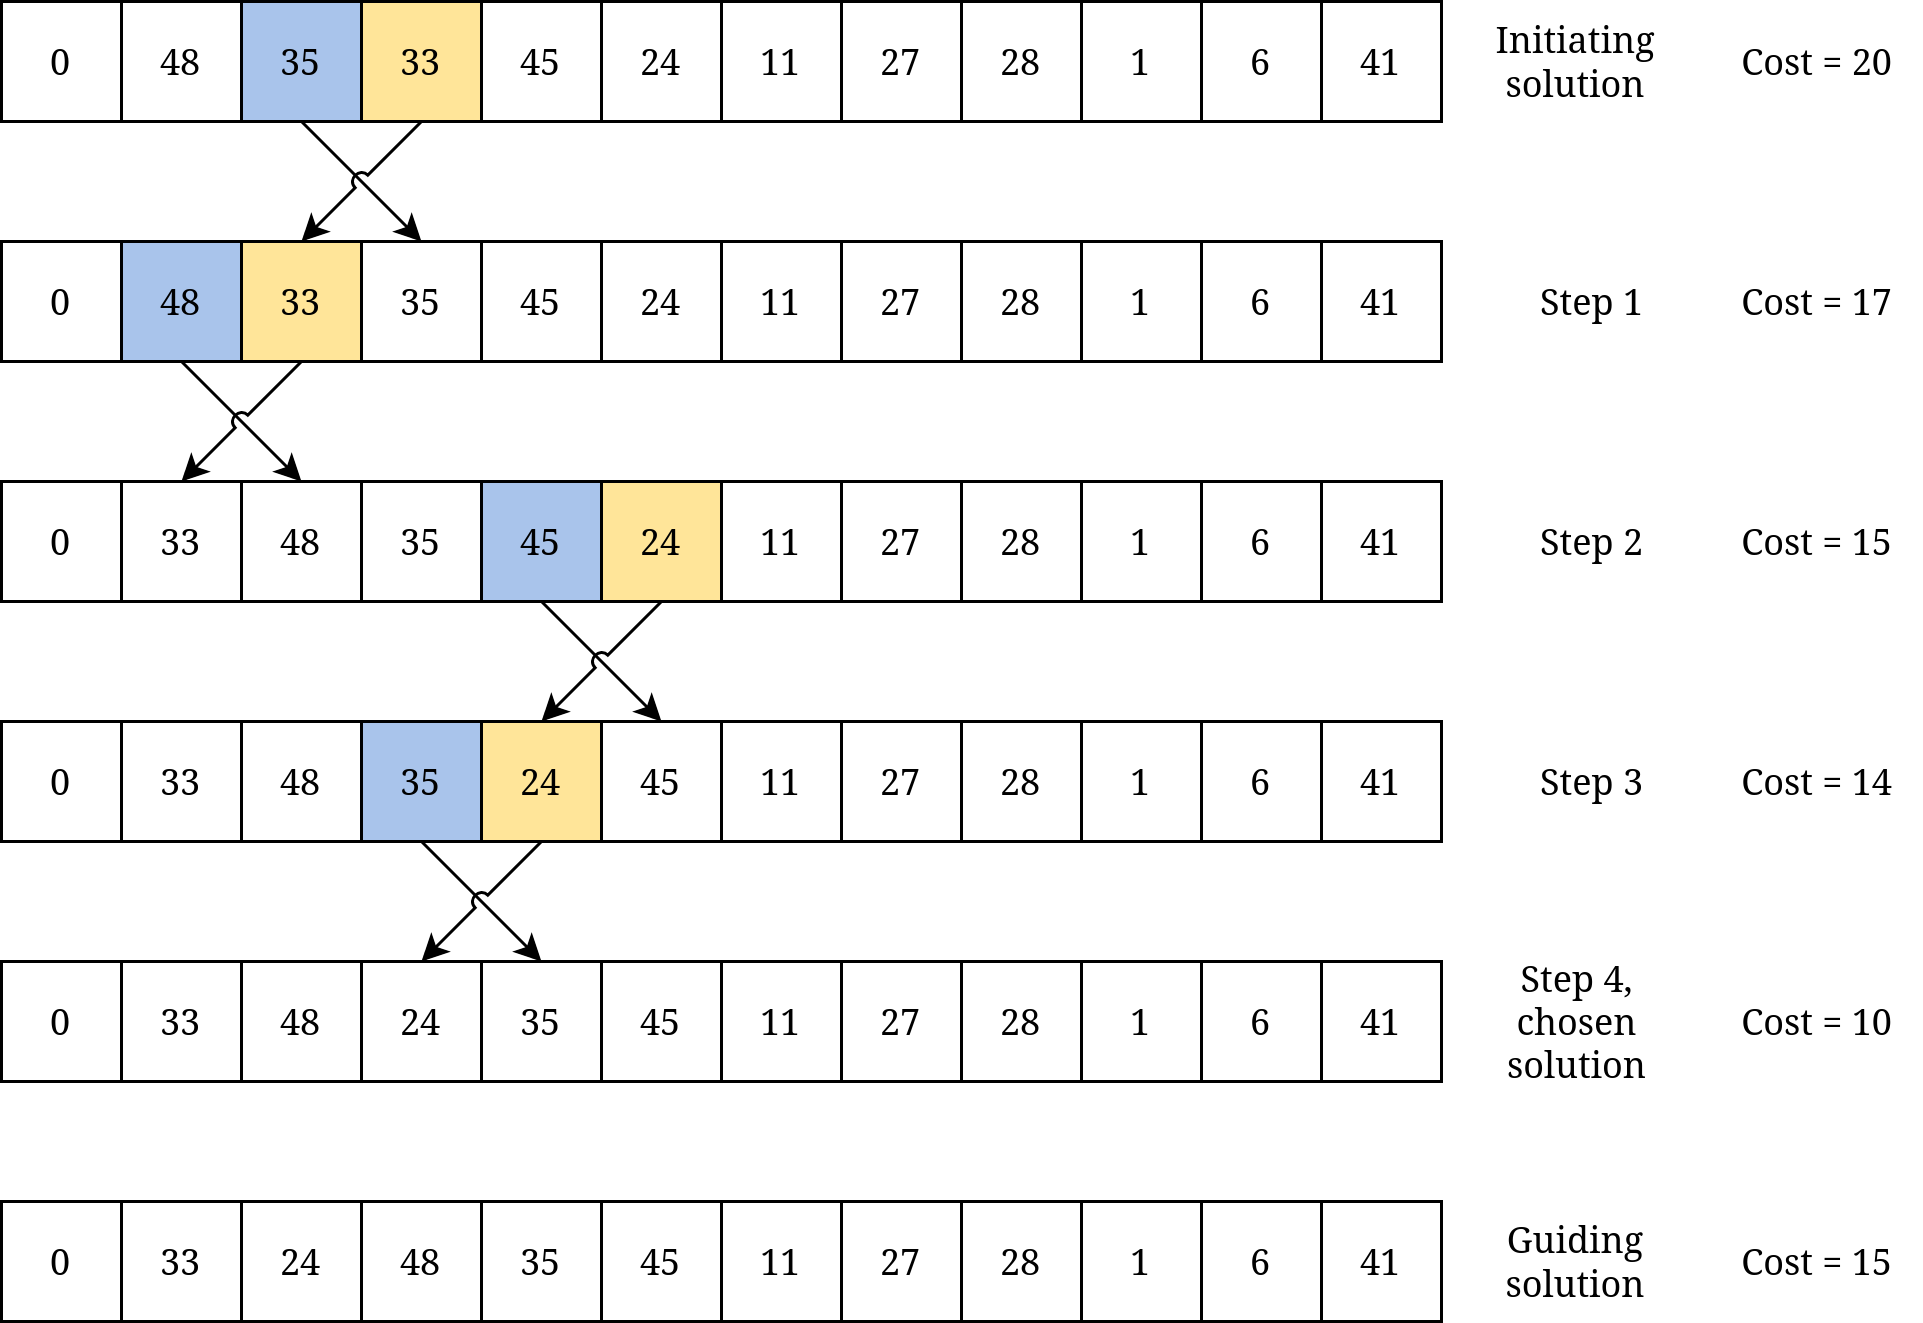
\includegraphics[width=0.45\textwidth]{images/path-relinker.png}
    \caption{Path-relinker algorithm sample} \label{Path-relinker algorithm sample}
\end{figure}

This operator aims to replace a PSO's particle's tendency towards their personal best and the global best.

\subsection{Swap operator}
For the PSO algorithm, the same swap + slide + reverse-swap operator as the genetic algorithm was used with remarkable success.
During the first implementation of the algorithm, only a simple swap of two elements was used as in figure \ref{Swap operation},
but the results it produced were 10-20\% worse overall. As an example, for the eil51 dataset with 2 salesmen, the simple swap operator
produced a mean value of 569, while the mean value for the swap + slide + reverse-swap operator was 489.

This operator aims to enhance PSO's exploration of the problem space by introducing more randomness with which 2-opt and
path-relinker can work.

\section{Results}
The algorithms were run using the following datasets:
\begin{enumerate}
    \item \texttt{eil51}, a 51-city MTSP problem by Christofides/Eilon
    \item \texttt{berlin51}, a 52-locations MTSP problem by Groetschel based on real-life Berlin, Germany
    \item \texttt{eil76}, a 76-city MTSP problem by Christofides/Eilon
    \item \texttt{rat99}, a 99-locations MTSP problem by Pulleyblank
\end{enumerate}

Each of the datasets was run with $n \in \{2, 3, 5\}$ salesmen. The runs were executed on a machine with an Intel Core i7
1260p processor at a constant frequency of 2GHz, using 10 of the 12 physical cores available. The algorithms can run on as
little as 1GB of RAM. In order to achieve good timings, the CPU should run on as a high frequency as it can achieve, as the
algorithms are compute-intensive.

The results of the runs can be seen in tables \ref{Fitness results for the genetic algorithm},
\ref{Runtime results for the genetic algorithm} for the genetic algorithm and tables
\ref{Fitness results for the particle swarm optimisation algorithm}, \ref{Runtime results for the particle swarm optimisation algorithm}
for the PSO, and visualisations are available on figures \ref{eil52, 3 salesmen}, \ref{eil52, 5 salesmen}, \ref{berlin52, 3 salesmen},
\ref{berlin52, 5 salesmen}, \ref{eil76, 3 salesmen}, \ref{eil76, 5 salesmen}, \ref{rat99, 3 salesmen} and \ref{rat99, 5 salesmen}
on the next pages.

\section{Discussions}
The two algorithms detailed in this paper were successful in finding near-optimal results for the MTSP problem datasets used
in this paper. Their runtimes - albeit high from a normal user perspective - exhibit a notable reduction in comparison when
compared to those of the CPLEX algorithm (GA 1m36s, PSO 4m45s, CPLEX 10080m for \texttt{rat99}, $n = 5$ salesmen). In this paper,
the Genetic algorithm provided better results, was faster overall and needed far fewer modifications to work with combinatorial
data. As for the particle swarm optimisation algorithm, the runtime was higher, but the results were comparable to the genetic
algorithm.

\section{Conclusions}
Optimisation algorithms like Genetic Algorithms and Particle Swarm Optimisation - often used for numerical function optimisation -
can be used for combinatorial function optimisation like MTSP with some modifications. The results of running the alforementioned
algorithms on combinatorial functions are often near-optimal, all while showing superior time efficiency.

The algorithms can further be improved through stochastic hyperparameter tuning and through hybridisation. In literature, there were
attempts to hybridise the Ant Colony Optimisation algorithm with the 2-opt operator \cite{b12} and to hybridise a particle swarm
optimisation algorithm using the GRASP algorithm \cite{b8} with good results.

\begin{thebibliography}{00}
    \bibitem{b1} O. Cheikhrouhou, I. Khoufi (2021). ``A comprehensive survey on the Multiple Traveling Salesman Problem: Applications, approaches and taxonomy''. Computer Science Review, 40, 100369. doi: 10.1016/j.cosrev.2021.1003.
    \bibitem{b2} L. Henri, E. Croitoru (2022). ``Genetic algorithms''. Faculty of Computer Science of University ``Alexandru Ioan Cuza'' of Iași.
    \bibitem{b3} S. Mirjalili (2018). ``Particle Swarm Optimisation. Evolutionary Algorithms and Neural Networks''. 15-31. doi: 10.1007/978-3-319-93025-1\_2.
    \bibitem{b4} M. A. Al-Furhud, Z. H. Ahmed (2020). ``Experimental Study of a Hybrid Genetic Algorithm for the Multiple Travelling Salesman Problem''. Mathematical Problems in Engineering, vol. 2020, p. 3431420. doi: 10.1155/2020/3431420.
    \bibitem{b5} \url{https://profs.info.uaic.ro/~mtsplib/MinMaxMTSP/index.html}
    \bibitem{b6} P. Singamsetty, J. K. Thenepalledoi (2021). ``An efficient genetic algorithm for solving open multiple travelling salesman problem with load balancing constraint''. Department of Mathematics, School of Advanced Sciences, VIT, Vellore-632014, Tamil Nadu, India. doi: 10.5267/j.dsl.2021.5.003
    \bibitem{b7} D. R. Singh, M. K. Singh, T. Singh, R. Prasad (2018). ``Genetic algorithm for solving multiple traveling salesmen problem using a new crossover and population generation''. Computación y Sistemas, 22(2).
    \bibitem{b8} S. D. Gulcu, H. K. Ornek (2019). ``Solution of Multiple Travelling Salesman Problem using Particle Swarm Optimization based Algorithms''. International Journal of Intelligent Systems and Applications in Engineering. ISSN: 2147-6799
    \bibitem{b9} \url{https://en.wikipedia.org/wiki/2-opt}
    \bibitem{b10} B. Penga, Zhipeng Lü, T.C.E. Cheng (2014). ``A Tabu Search/Path Relinking Algorithm to Solve the Job Shop Scheduling Problem''. hool of Computer Science and Technology, Huazhong University of Science and Technology, Wuhan, 430074, P.R. China. doi: 10.48550/arXiv.1402.5613
    \bibitem{b11} C. C. C. Ribeiro, M. G. C. Resend (2010). ``Path-relinking intensification methods for stochastic Local Search Algorithms''. Department of Computer Science, Universidade Federal Fluminense, Rua Passo da Pátria, 156, Niteráoi, RJ 24210-240 Brazil. URL: \url{https://mauricio.resende.info/doc/spr.pdf}
    \bibitem{b12} K. Saraswathi, A. Tamilarasi (2016). ``Ant Colony Optimization Based Feature Selection for Opinion Mining Classification''.  Journal of Medical Imaging and Health Informatics, Volume 6. doi: 10.1166/jmihi.2016.1856
\end{thebibliography}


\begin{table*}[h]
    \centering
    \begin{tabular}{|c|c|c|c|c|c|}
        \hline 
        Dataset & Dimensions & Best cost [min, max] & Median cost [min, max] & Worst cost [min, max] \\
        \hline
        & 2 & 452.4917, [205.7164, 246.7753] & 489.3968, [242.2249, 247.1719] & 515.7682, [221.6817, 294.0865] \\
        eil51 & 3 & 498.3084, [156.9638, 183.4012] & 518.9448, [160.8375, 184.4372] & 566.9566, [161.5549, 207.9621] \\
        & 5 & 572.3836, [77.3725, 131.3495] & 661.8094, [101.8904, 150.5947] & 733.4215, [68.8432, 183.4685] \\
        \hline
        & 2 & 8201.6263, [2595.4587, 5606.1676] & 8590.6848, [2697.2115, 5893.4733] & 9307.7586, [2992.1265, 6315.6321] \\
        berlin52 & 3 & 8996.8522, [2115.4115, 4001.3250] & 9594.4198, [1223.1735, 4365.7421] & 10863.9695, [1867.7822, 4966.9029] \\
        & 5 & 10892.5415, [578.9702, 3015.3396] & 11556.2447, [931.1152, 2959.9547] & 11912.2920, [700.1437, 2974.0190] \\
        \hline
        & 2 & 581.0691, [276.2812, 304.7880] & 622.9683, [300.8131, 322.1552] & 670.6645, [289.7983, 380.8662] \\
        eil76 & 3 & 638.9018, [195.2157, 222.1578] & 687.3440, [189.9131, 252.9988] & 737.6305, [180.3664, 292.0079] \\
        & 5 & 801.1751, [131.5410, 170.4222] & 878.9306, [125.3454, 189.6171] & 947.2019, [119.7203, 219.1424] \\
        \hline
        & 2 & 1478.4560, [726.2807, 752.1753] & 1564.7694, [778.9769, 785.7925] & 1641.2690, [799.5244, 841.7446] \\
        rat99 & 3 & 1738.7757, [561.4327, 610.7246] & 1873.4486, [604.1806, 644.0537] & 1936.9353, [581.5455, 680.7555] \\
        & 5 & 2419.9191, [404.0482, 520.0018] & 2569.2387, [410.6488, 548.4963] & 2757.0272, [456.9319, 604.7306] \\
        \hline
    \end{tabular}
    \captionof{figure}{Fitness results for the genetic algorithm} \label{Fitness results for the genetic algorithm}
\end{table*}

\begin{table*}[h]
    \centering
    \begin{tabular}{|c|c|c|c|c|c|}
        \hline 
        Dataset & Dimensions & Best time (seconds) & Median time (seconds) & Worst time (seconds) \\
        \hline
        & 2 & 35.0730 & 39.3025 & 40.2845 \\
        eil51 & 3 & 36.6657 & 40.6693 & 40.9740 \\
        & 5 & 38.3636 & 40.4140 & 42.9961 \\
        \hline
        & 2 & 35.8471 & 40.5474 & 40.7477 \\
        berlin52 & 3 & 36.7146 & 41.5331 & 42.1390 \\
        & 5 & 38.5821 & 43.4023 & 44.1265 \\
        \hline
        & 2 & 59.2793 & 62.9946 & 63.8993 \\
        eil76 & 3 & 61.3011 & 64.2504 & 65.2739 \\
        & 5 & 62.8406 & 66.3060 & 67.2039 \\
        \hline
        & 2 & 88.9989 & 91.9548 & 93.5630 \\
        rat99 & 3 & 88.7005 & 93.2481 & 94.1409 \\
        & 5 & 90.4842 & 94.3258 & 96.2429 \\
        \hline
    \end{tabular}
    \captionof{figure}{Runtime results for the genetic algorithm} \label{Runtime results for the genetic algorithm}
\end{table*}

\begin{table*}[h]
    \centering
    \begin{tabular}{|c|c|c|c|c|c|}
        \hline 
        Dataset & Dimensions & Best cost [min, max] & Median cost [min, max] & Worst cost [min, max] \\
        \hline
        & 2 & 449.7163 [214.1512, 235.5651] & 475.5942, [192.9591, 282.6351] & 499.3102, [244.9411, 254.3691] \\
        eil51 & 3 & 489.5325, [157.1746, 166.5948] & 531.2806, [142.3028, 196.6333] & 578.3335, [181.7417, 201.7480] \\
        & 5 & 640.2244, [88.7013, 146.2878] & 697.6553, [102.2351, 153.4138] & 784.5660, [117.1869, 173.1557] \\
        \hline
        & 2 & 7976.8215, [2996.0896, 4980.7319] & 8415.4363, [2969.9692, 5445.4672] & 8647.5823, [4186.8835, 4460.6987] \\
        berlin52 & 3 & 8771.5855, [2360.1379, 3811.5594] & 9661.0789, [3082.9605, 3393.0226] & 10190.7955, [2871.2697, 3782.7879] \\
        & 5 & 11253.1301, [577.7584, 3023.0627] & 12362.8712, [1312.6386, 3029.0983] & 13593.6078, [1099.0985, 3678.7885] \\
        \hline
        & 2 & 582.0823, [267.7988, 314.2835] & 609.2940, [258.9784, 350.3156] & 639.0766, [306.9239, 332.1527] \\
        eil76 & 3 & 650.3413, [188.5105, 235.7174] & 682.4711, [188.3825, 247.9872] & 741.4631, [234.9759, 256.2703] \\
        & 5 & 836.9620, [127.3422, 187.9968] & 949.0180, [142.0018, 209.3440] & 967.5711, [161.3675, 222.9497] \\
        \hline
        & 2 & 1404.4009, [677.7814, 726.6194] & 1466.0078, [708.4931, 757.5147] & 1530.4149, [761.7108, 768.7042] \\
        rat99 & 3 & 1705.9939, [436.4255, 666.6766] & 1814.2634, [514.3615, 672.1688] & 1968.9282, [620.0822, 677.6363] \\
        & 5 & 2460.4928, [327.3417, 574.1595] & 2662.7770, [436.9524, 586.0860] & 2779.0884, [436.0260, 609.4613] \\
        \hline
    \end{tabular}
    \captionof{figure}{Fitness results for the particle swarm optimisation algorithm} \label{Fitness results for the particle swarm optimisation algorithm}
\end{table*}

\begin{table*}[h]
    \centering
    \begin{tabular}{|c|c|c|c|c|c|}
        \hline 
        Dataset & Dimensions & Best time (seconds) & Median time (seconds) & Worst time (seconds) \\
        \hline
        & 2 & 60.0396 & 86.3428 & 101.1629 \\
        eil51 & 3 & 47.5369 & 61.4150 & 76.4317 \\
        & 5 & 36.8183 & 48.7286 & 61.3814 \\
        \hline
        & 2 & 63.2038 & 91.6510 & 103.4645 \\
        berlin52 & 3 & 48.7222 & 59.6309 & 84.4854 \\
        & 5 & 43.3237 & 54.1800 & 62.8043 \\
        \hline
        & 2 & 187.6626 & 238.9693 & 287.5738 \\
        eil76 & 3 & 145.2984 & 180.1258 & 215.3485 \\
        & 5 & 110.0897 & 140.1826 & 165.7784 \\
        \hline
        & 2 & 363.4923 & 511.2023 & 552.7536 \\
        rat99 & 3 & 281.8676 & 348.8739 & 430.0076 \\
        & 5 & 211.3089 & 288.1322 & 1411.9221 \\
        \hline
    \end{tabular}
    \captionof{figure}{Runtime results for the particle swarm optimisation algorithm} \label{Runtime results for the particle swarm optimisation algorithm}
\end{table*}

\begin{figure*}[h]
    \centering
    \begin{subfigure}{.5\textwidth}
      \centering
      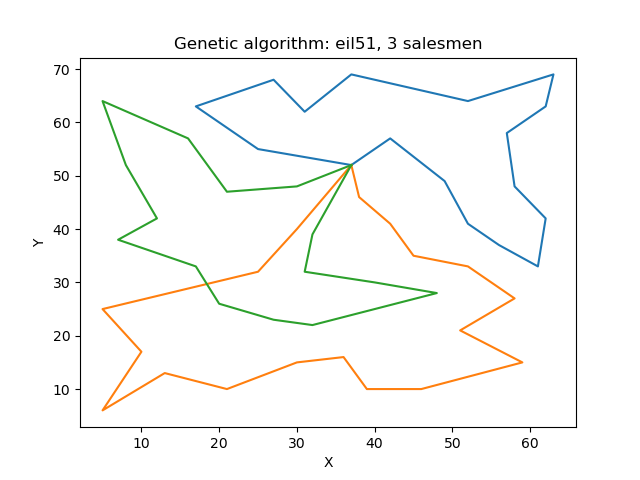
\includegraphics[width=\textwidth]{images/Genetic algorithm: eil51, 3 salesmen.png}
    \end{subfigure}%
    \begin{subfigure}{.5\textwidth}
      \centering
      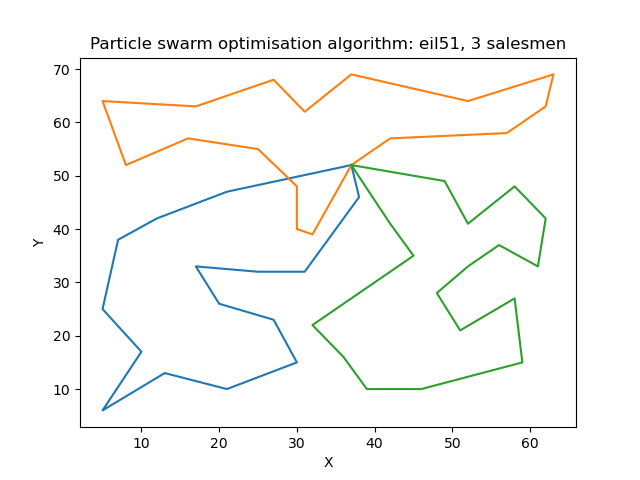
\includegraphics[width=\textwidth]{images/Particle swarm optimisation algorithm: eil51, 3 salesmen.png}
    \end{subfigure}%
    \caption{\texttt{eil52}, 3 salesmen} \label{eil52, 3 salesmen}
\end{figure*}

\begin{figure*}[h]
    \centering
    \begin{subfigure}{.5\textwidth}
      \centering
      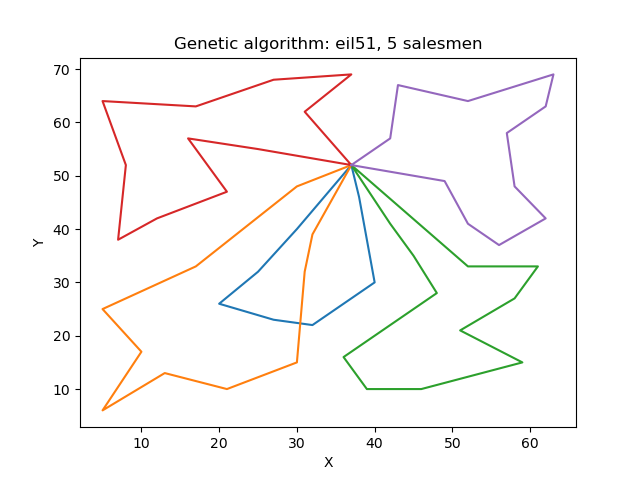
\includegraphics[width=\textwidth]{images/Genetic algorithm: eil51, 5 salesmen.png}
    \end{subfigure}%
    \begin{subfigure}{.5\textwidth}
      \centering
      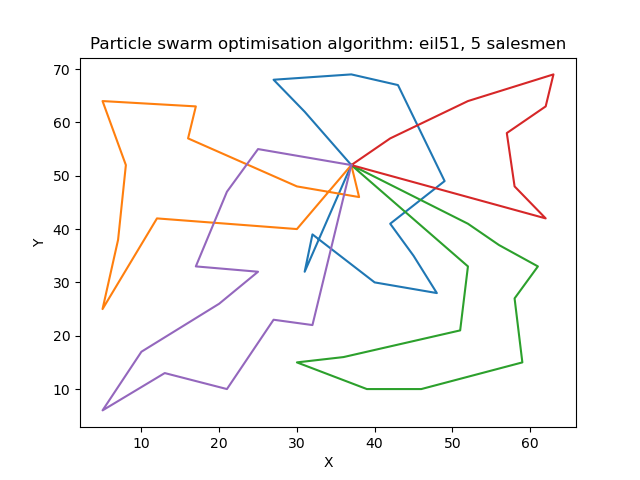
\includegraphics[width=\textwidth]{images/Particle swarm optimisation algorithm: eil51, 5 salesmen.png}
    \end{subfigure}%
    \caption{\texttt{eil52}, 3 salesmen} \label{eil52, 5 salesmen}
\end{figure*}

\begin{figure*}[h]
    \centering
    \begin{subfigure}{.5\textwidth}
      \centering
      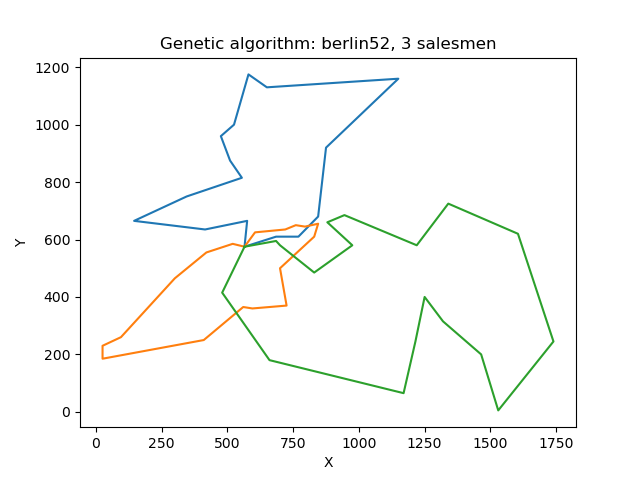
\includegraphics[width=\textwidth]{images/Genetic algorithm: berlin52, 3 salesmen.png}
    \end{subfigure}%
    \begin{subfigure}{.5\textwidth}
      \centering
      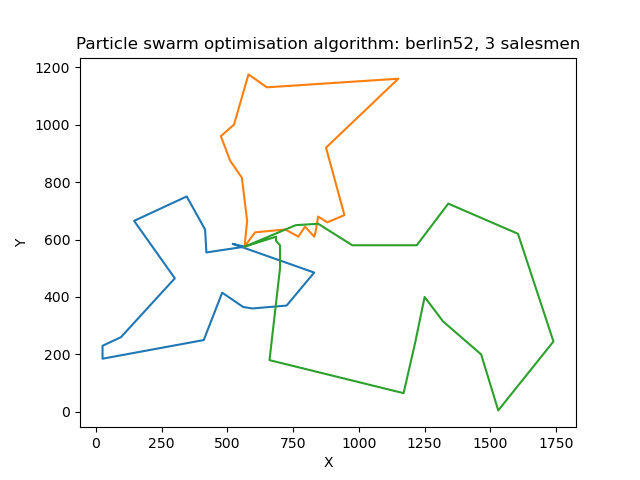
\includegraphics[width=\textwidth]{images/Particle swarm optimisation algorithm: berlin52, 3 salesmen.png}
    \end{subfigure}%
    \caption{\texttt{berlin52}, 3 salesmen} \label{berlin52, 3 salesmen}
\end{figure*}

\begin{figure*}[h]
    \centering
    \begin{subfigure}{.5\textwidth}
      \centering
      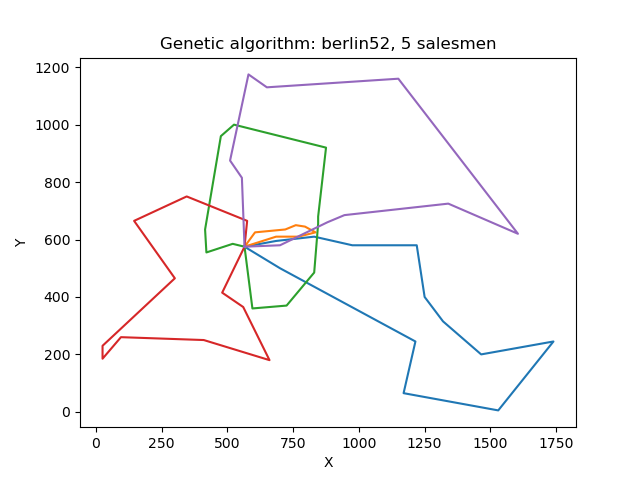
\includegraphics[width=\textwidth]{images/Genetic algorithm: berlin52, 5 salesmen.png}
    \end{subfigure}%
    \begin{subfigure}{.5\textwidth}
      \centering
      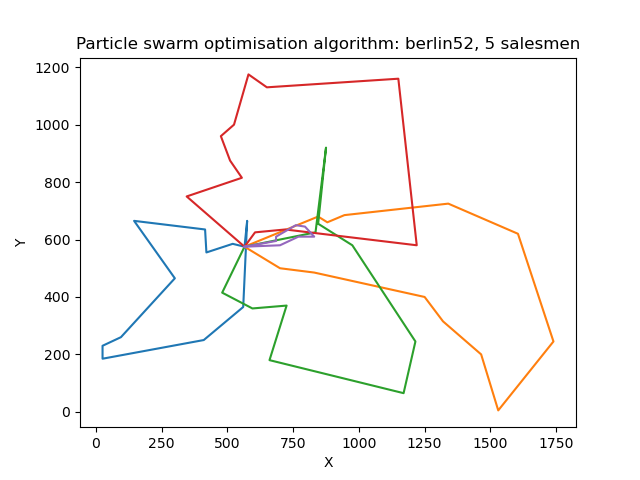
\includegraphics[width=\textwidth]{images/Particle swarm optimisation algorithm: berlin52, 5 salesmen.png}
    \end{subfigure}%
    \caption{\texttt{berlin52}, 5 salesmen} \label{berlin52, 5 salesmen}
\end{figure*}

\begin{figure*}[h]
    \centering
    \begin{subfigure}{.5\textwidth}
      \centering
      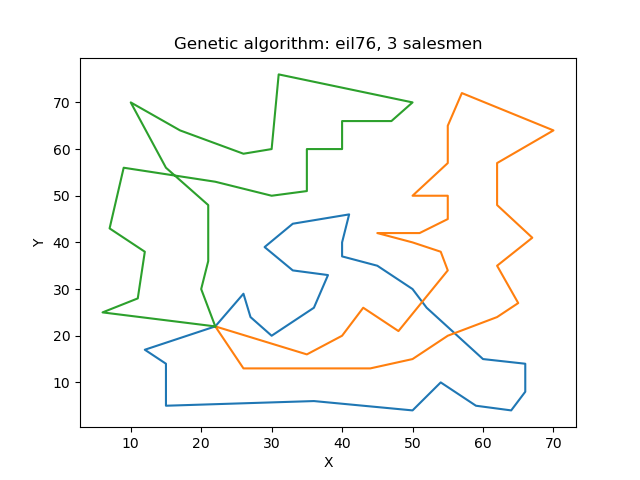
\includegraphics[width=\textwidth]{images/Genetic algorithm: eil76, 3 salesmen.png}
    \end{subfigure}%
    \begin{subfigure}{.5\textwidth}
      \centering
      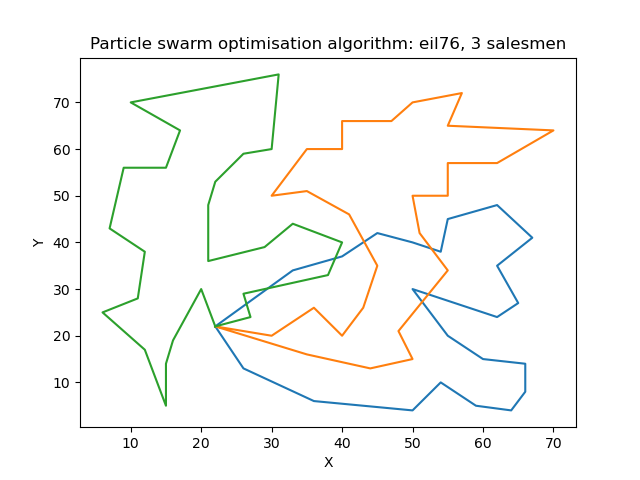
\includegraphics[width=\textwidth]{images/Particle swarm optimisation algorithm: eil76, 3 salesmen.png}
    \end{subfigure}%
    \caption{\texttt{eil76}, 3 salesmen} \label{eil76, 3 salesmen}
\end{figure*}

\begin{figure*}[h]
    \centering
    \begin{subfigure}{.5\textwidth}
      \centering
      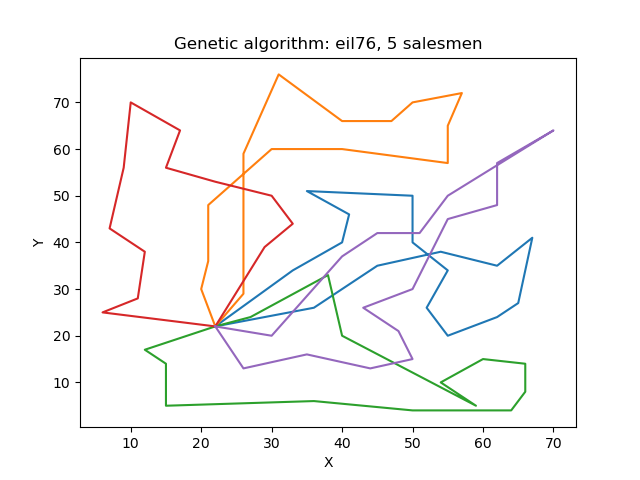
\includegraphics[width=\textwidth]{images/Genetic algorithm: eil76, 5 salesmen.png}
    \end{subfigure}%
    \begin{subfigure}{.5\textwidth}
      \centering
      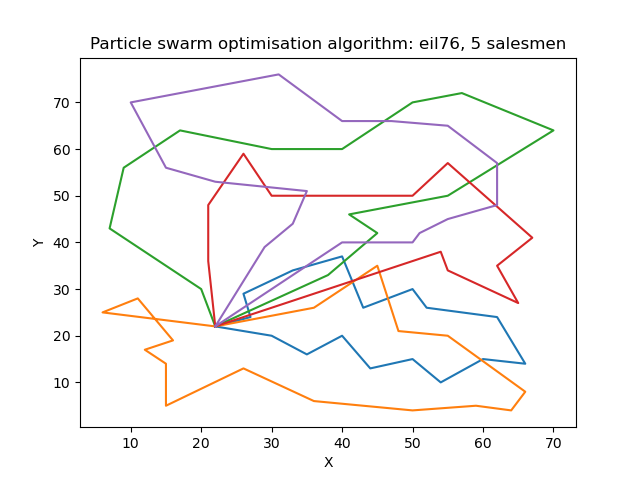
\includegraphics[width=\textwidth]{images/Particle swarm optimisation algorithm: eil76, 5 salesmen.png}
    \end{subfigure}%
    \caption{\texttt{eil76}, 5 salesmen} \label{eil76, 5 salesmen}
\end{figure*}

\begin{figure*}[h]
    \centering
    \begin{subfigure}{.5\textwidth}
      \centering
      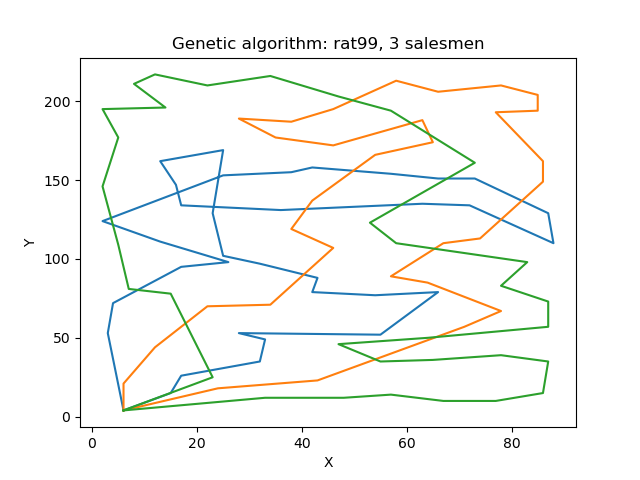
\includegraphics[width=\textwidth]{images/Genetic algorithm: rat99, 3 salesmen.png}
    \end{subfigure}%
    \begin{subfigure}{.5\textwidth}
      \centering
      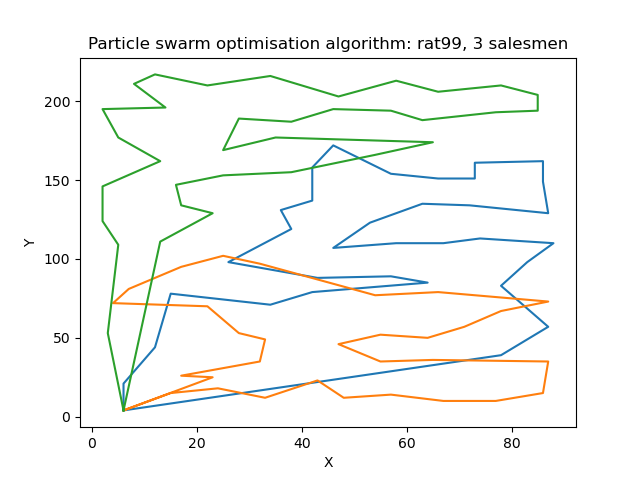
\includegraphics[width=\textwidth]{images/Particle swarm optimisation algorithm: rat99, 3 salesmen.png}
    \end{subfigure}%
    \caption{\texttt{rat99}, 3 salesmen} \label{rat99, 3 salesmen}
\end{figure*}

\begin{figure*}[h]
    \centering
    \begin{subfigure}{.5\textwidth}
      \centering
      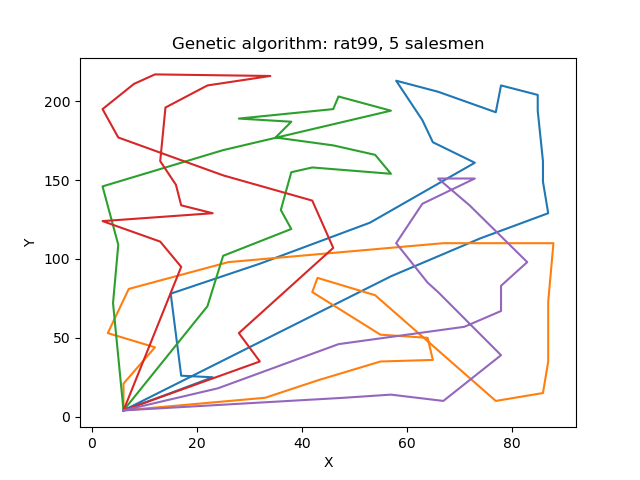
\includegraphics[width=\textwidth]{images/Genetic algorithm: rat99, 5 salesmen.png}
    \end{subfigure}%
    \begin{subfigure}{.5\textwidth}
      \centering
      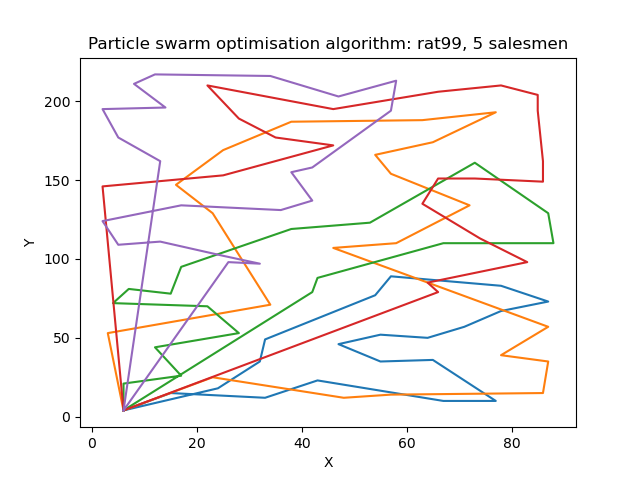
\includegraphics[width=\textwidth]{images/Particle swarm optimisation algorithm: rat99, 5 salesmen.png}
    \end{subfigure}%
    \caption{\texttt{rat99}, 5 salesmen} \label{rat99, 5 salesmen}
\end{figure*}

\end{document}
